\documentclass[border=6pt]{standalone}
\usepackage[T1]{fontenc}
\usepackage{amsmath,amssymb}
\usepackage{tikz}
\usetikzlibrary{arrows.meta,positioning,calc}
\usepackage{fontawesome5}
\begin{document}
\scalebox{2.6}{%
\begin{tikzpicture}[
			x=1cm,
			y=0.76cm,
			font=\tiny,
			>=Stealth,
			ris/.style={draw=green!55!black, fill=green!10, thick, minimum width=0.34cm, minimum height=0.82cm},
			cpu/.style={draw=black!65, fill=gray!10, rounded corners=1pt, thick, minimum width=1.05cm, minimum height=0.34cm, align=center},
			direct/.style={->, line width=0.42pt, blue!70!black},
			reflected/.style={->, line width=0.42pt, orange!85!black},
			fronthaul/.style={->, dashed, line width=0.42pt, gray!70!black},
			linklabel/.style={font=\tiny, fill=white, inner sep=0.8pt},
			bsicon/.style={text=blue!65!black, inner sep=0pt, font=\LARGE},
			ueicon/.style={text=orange!80!black, inner sep=0pt, font=\Large}
		]
			\node[bsicon] (bs1) at (0.60,2.48) {\faBroadcastTower};
			\node[bsicon] (bs2) at (3.00,2.08) {\faBroadcastTower};
			\node[bsicon] (bs3) at (5.40,2.48) {\faBroadcastTower};
			\node[ueicon] (ue1) at (0.80,0.52) {\faIcon{mobile-alt}};
			\node[ueicon] (ue2) at (3.00,0.44) {\faIcon{mobile-alt}};
			\node[ueicon] (ue3) at (5.20,0.52) {\faIcon{mobile-alt}};
			\node[cpu] (cpu) at (3.00,3.06) {CPU};
			\node[ris] (ris1) at (1.88,1.52) {};
			\node[ris] (ris2) at (4.12,1.52) {};

			\node[above=0.42cm of bs1, align=center] {BS 1};
			\node[anchor=west] at (3.30,2.50) {BS 2};
			\node[above=0.42cm of bs3, align=center] {BS $C$};

			\foreach \ue/\lab in {ue1/UE 1,ue2/UE 2,ue3/UE $K$}{
				\node[below=0.28cm of \ue] {\lab};
			}

			\foreach \r/\lab in {ris1/RIS 1,ris2/RIS $Q$}{
				\foreach \dy in {-0.30,-0.10,0.10,0.30}{
					\draw[green!55!black, line width=0.18pt] ($(\r.west)+(0,\dy)$) -- ($(\r.east)+(0,\dy)$);
				}
				\foreach \dx in {-0.08,0.08}{
					\draw[green!55!black, line width=0.18pt] ($(\r.south)+(\dx,0)$) -- ($(\r.north)+(\dx,0)$);
				}
				\node[below=0.18cm of \r, align=center] {\lab};
			}

			\draw[fronthaul] (bs1.north east) -- (cpu.south west);
			\draw[fronthaul] (bs2.north) -- (cpu.south);
			\draw[fronthaul] (bs3.north west) -- (cpu.south east);

			\draw[direct] (ue1.north) to[bend left=8] (bs1.south);
			\draw[direct] (ue2.north) to[bend left=6] (bs2.south);
			\draw[direct] (ue3.north) to[bend right=8] (bs3.south);
			\draw[reflected] (ue1.north east) to[bend left=6] (ris1.south west);
			\draw[reflected] (ue2.north west) to[bend right=6] (ris1.south east);
			\draw[reflected] (ris1.north west) to[bend left=8] (bs1.south east);
			\draw[reflected] (ris1.north east) to[bend right=8] (bs2.west);
			\draw[reflected] (ue2.north east) to[bend left=6] (ris2.south west);
			\draw[reflected] (ue3.north west) to[bend right=6] (ris2.south east);
			\draw[reflected] (ris2.north west) to[bend left=8] (bs2.east);
			\draw[reflected] (ris2.north east) to[bend left=8] (bs3.south west);
		
			% legend and impairment note (added for the website)
			\begin{scope}[shift={(0.35,-1.10)}]
				\draw[direct] (0,0) -- (0.40,0); \node[anchor=west] at (0.42,0) {direct link};
				\draw[reflected] (1.75,0) -- (2.15,0); \node[anchor=west] at (2.17,0) {RIS-reflected link};
				\draw[fronthaul] (4.30,0) -- (4.70,0); \node[anchor=west] at (4.72,0) {fronthaul};
			\end{scope}
			\node[draw=red!65!black, fill=red!6, rounded corners=1pt, inner sep=1.5pt, align=center]
				at (3.00,-1.75) {IQ imbalance at every UE (transmit) and BS (receive)};
		\end{tikzpicture}
}
\end{document}
